\section[aplikace]{Aplikace}

\begin{figure}[h]
    \begin{center}
        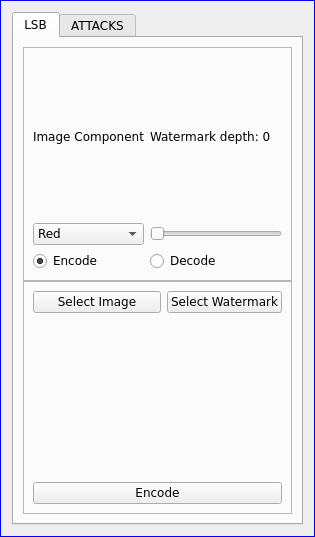
\includegraphics[scale=0.5]{images/app.jpg}
        \caption{Aplikace po spuštění}
    \end{center}
\end{figure}

Po spuštění aplikace je možné vložit/extrahovat LSB vodoznak do/z obrázku, nebo zkusit nějaký útok na již vodoznačený obrázek.

\section[lsb]{LSB Vodoznačení}

Pro vytvoření vodoznaku je třeba vybrat jakou složku obrazu využít na vodoznak a do jaké bitové hloubky bude vodoznak zasazen. Dále je třeba vybrat obrázek, který bude vodoznačen a samotný vodoznak. Pokud je vodoznak menší, než původní obrázek bude zduplikován tak, aby vyplnil celý rozsah.

\begin{figure}[h!]
    \begin{center}
        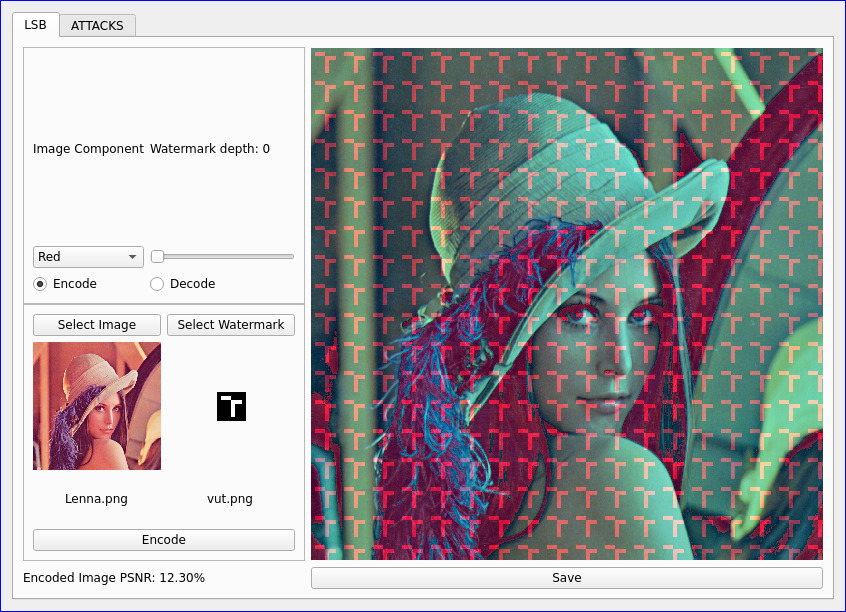
\includegraphics[scale=0.4]{images/encoding.jpg}
        \caption{Vytvoření LSB vodoznaku}
    \end{center}
\end{figure}

\begin{figure*}[h!]
    \begin{center}
        \begin{subfigure}[t]{0.5\textwidth}
            \centering
            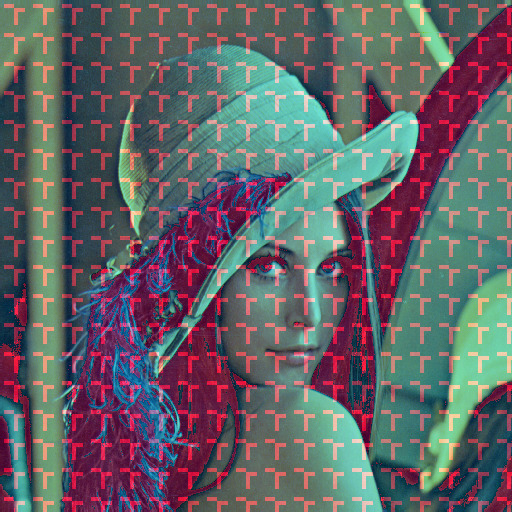
\includegraphics[height=8cm]{images/lsb_0.jpg}
            \caption{LSB v minimální hloubce}
        \end{subfigure}%
        ~
        \begin{subfigure}[t]{0.5\textwidth}
            \centering
            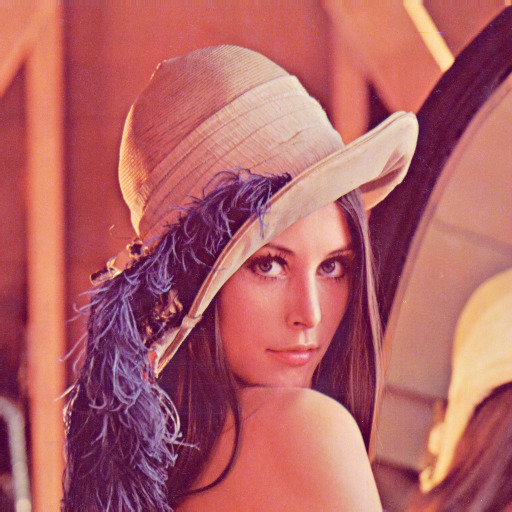
\includegraphics[height=8cm]{images/lsb_7.jpg}
            \caption{LSB v maximální hloubce}
        \end{subfigure}
        \caption{Rozdíly v hloubkách u LSB}
    \end{center}
\end{figure*}


\clearpage


Pro extrakci vodoznaku stačí pouze vybrat obrázek, složku a hloubku.

\begin{figure}[h!]
    \begin{center}
        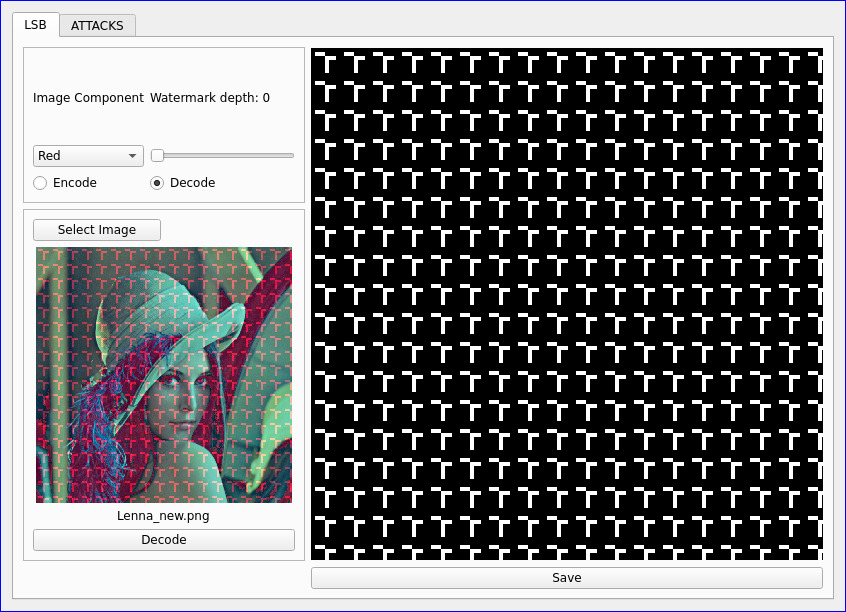
\includegraphics[scale=0.4]{images/decoding.jpg}
        \caption{Extrakce LSB vodoznaku}
    \end{center}
\end{figure}

\newpage
\section[utoky]{Útoky}
V aplikaci jsou implementovány 4 typy útoků:
\begin{itemize}
    \item JPEG Komprese
    \item Rotace a následné vrácení zpět
    \item Zmenšení velikosti
    \item Zrcadlení obrázku
\end{itemize}

\begin{figure}[h!]
    \begin{center}
        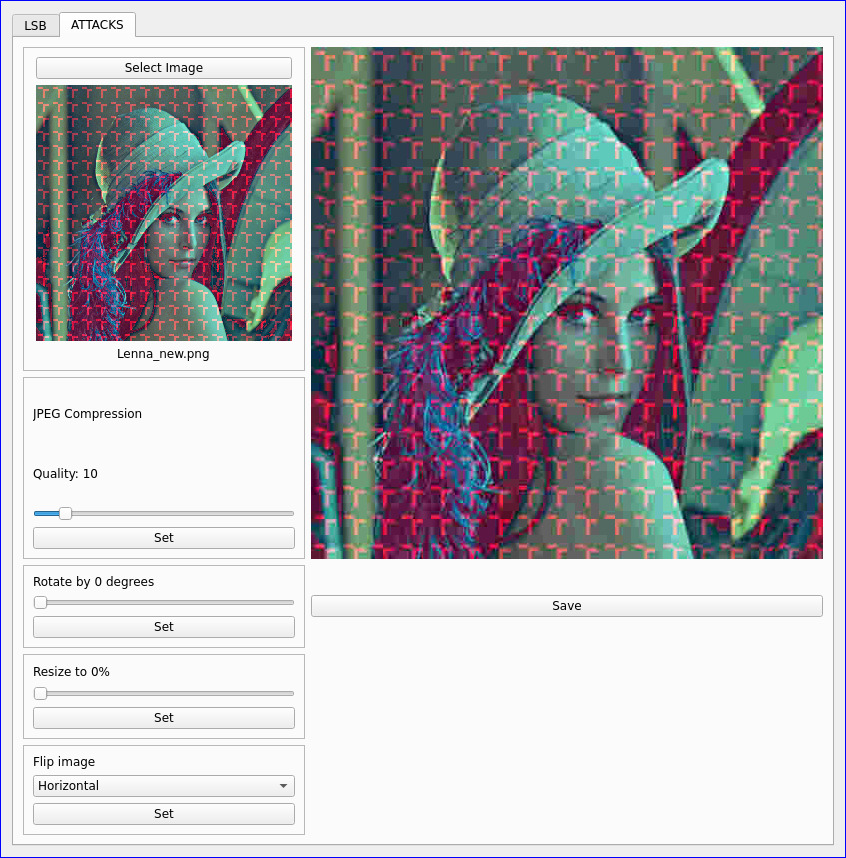
\includegraphics[scale=0.4]{images/attacks.jpg}
        \caption{Útoky na vodoznak}
    \end{center}
\end{figure}

\subsection[jpeg]{JPEG Komprese obrázku}
Komprese je velmi účinná proti vodoznaku ve velké hloubce. I velmi malá komprese dokáže vodoznak úplně zničit.

\begin{figure*}[h!]
    \begin{center}
        \begin{subfigure}[t]{0.5\textwidth}
            \centering
            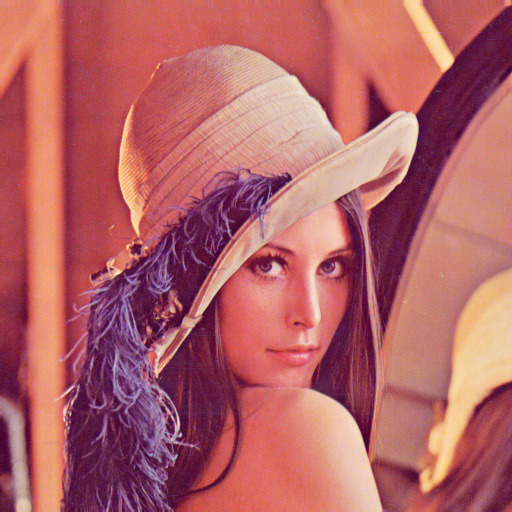
\includegraphics[height=8cm]{images/lsb_7_95_qual.jpg}
            \caption{LSB v maximální hloubce po JPEG kompresi s 95\% kvalitou}
        \end{subfigure}%
        ~
        \begin{subfigure}[t]{0.5\textwidth}
            \centering
            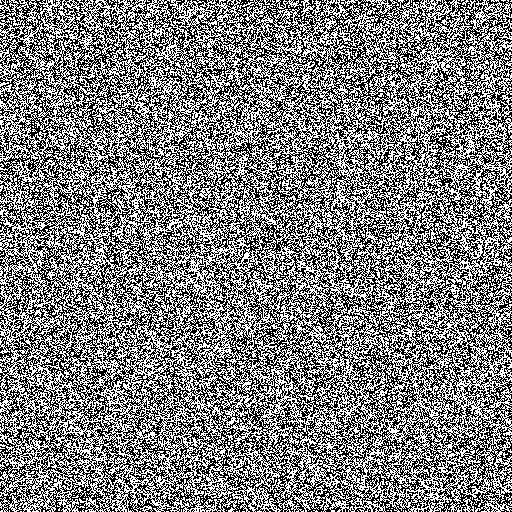
\includegraphics[height=8cm]{images/lsb_7_95_qual_extracted.jpg}
            \caption{Extrahovaný obrázek}
        \end{subfigure}
        \caption{Vliv komprese na maximální hloubku vodoznaku}
    \end{center}
\end{figure*}

\begin{figure*}[h!]
    \begin{center}
        \begin{subfigure}[t]{0.5\textwidth}
            \centering
            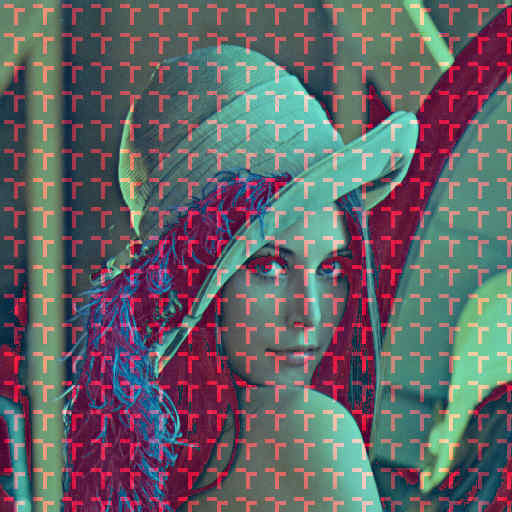
\includegraphics[height=8cm]{images/lsb_0_35_qual.jpg}
            \caption{LSB v minimální hloubce po JPEG kompresi s 35\% kvalitou}
        \end{subfigure}%
        ~
        \begin{subfigure}[t]{0.5\textwidth}
            \centering
            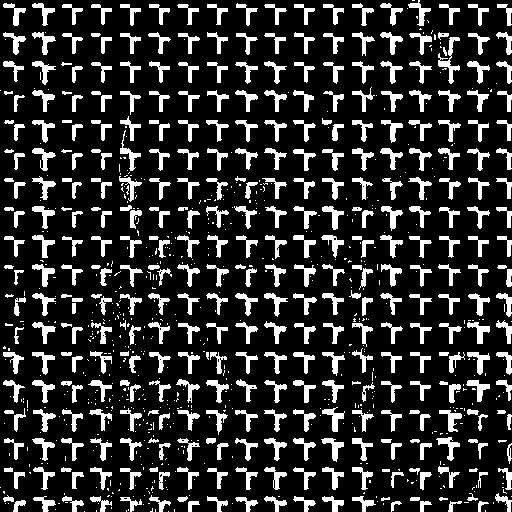
\includegraphics[height=8cm]{images/lsb_0_35_qual_extracted.jpg}
            \caption{Extrahovaný obrázek}
        \end{subfigure}
        \caption{Vliv komprese na minimální hloubku vodoznaku}
    \end{center}
\end{figure*}

\clearpage

\subsection[rotace]{Rotace obrázku}
Rotace je implementována tak, že obrázek se při první rotaci zvětší tak, aby mu nebyly oříznuty rohy a po rotaci zpět je oříznut zpět na původní velikost. Z tohoto důvodu nemá rotace velký vliv na extrahovaný vodoznak, pouze do něj vnese drobný šum.

\begin{figure}[h!]
    \begin{center}
        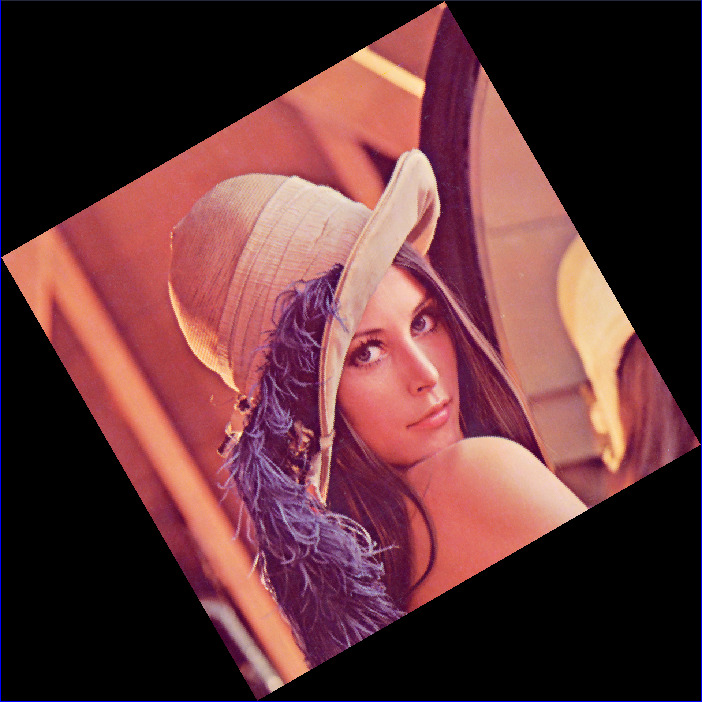
\includegraphics[scale=0.4]{images/rotation_30deg.jpg}
        \caption{Obrázek po první rotaci}
    \end{center}
\end{figure}

\begin{figure*}[h!]
    \begin{center}
        \begin{subfigure}[t]{0.5\textwidth}
            \centering
            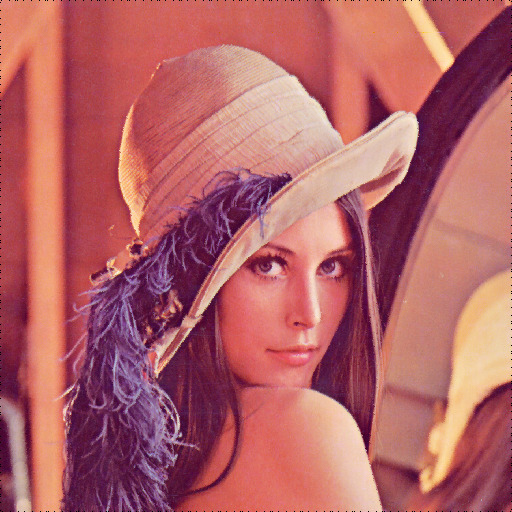
\includegraphics[height=8cm]{images/rotation_30deg_fin.jpg}
            \caption{Obrázek po rotaci o 30\textdegree{}, zpět a po oříznutí okrajů}
        \end{subfigure}%
        ~
        \begin{subfigure}[t]{0.5\textwidth}
            \centering
            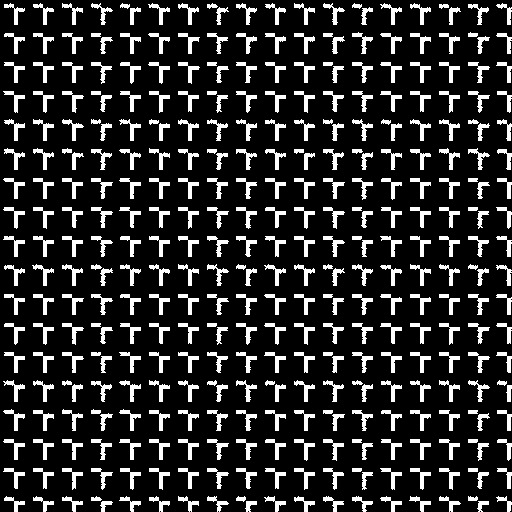
\includegraphics[height=8cm]{images/rotation_30deg_extracted.jpg}
            \caption{Extrahovaný obrázek}
        \end{subfigure}
        \caption{Vliv rotace na vodoznak}
    \end{center}
\end{figure*}

\clearpage
\subsection[zmenseni]{Zmenšení velikosti obrázku}
Podobně jako JPEG komprese, i změna velikosti obrázku výrazně ovlivňuje vodoznak.

\begin{figure*}[h!]
    \begin{center}
        \begin{subfigure}[t]{0.5\textwidth}
            \centering
            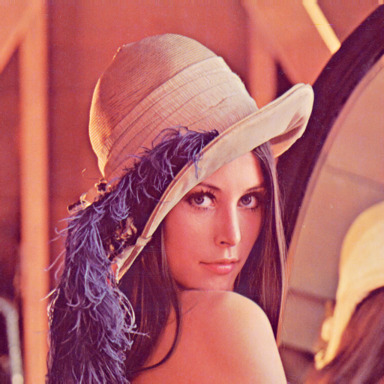
\includegraphics[height=8cm]{images/resize_7_75percent.jpg}
            \caption{Obrázek po zmenšení na 75\%}
        \end{subfigure}%
        ~
        \begin{subfigure}[t]{0.5\textwidth}
            \centering
            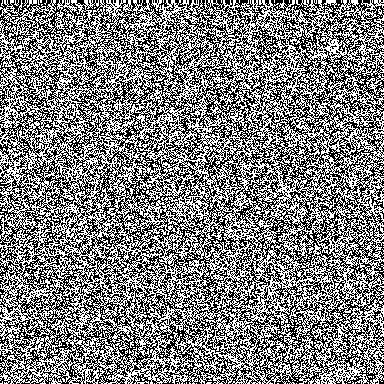
\includegraphics[height=8cm]{images/resize_7_75percent_extracted.jpg}
            \caption{Extrahovaný obrázek}
        \end{subfigure}
        \caption{Vliv zmenšení na vodoznak v maximální hloubce}
    \end{center}
\end{figure*}

\begin{figure*}[h!]
    \begin{center}
        \begin{subfigure}[t]{0.5\textwidth}
            \centering
            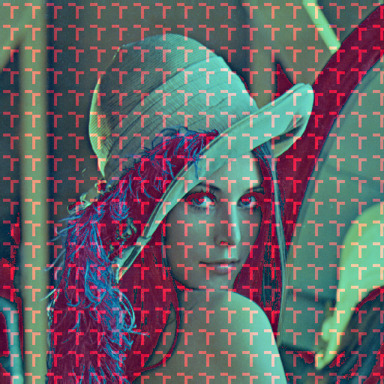
\includegraphics[height=8cm]{images/resize_0_75percent.jpg}
            \caption{Obrázek po zmenšení na 75\%}
        \end{subfigure}%
        ~
        \begin{subfigure}[t]{0.5\textwidth}
            \centering
            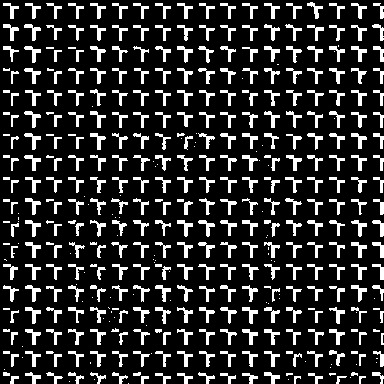
\includegraphics[height=8cm]{images/resize_0_75percent_extracted.jpg}
            \caption{Extrahovaný obrázek}
        \end{subfigure}
        \caption{Vliv zmenšení na vodoznak v minimální hloubce}
    \end{center}
\end{figure*}

\clearpage
\subsection[zrcadleni]{Zrcadlení obrázku}
Zrcadlení obrázku nemá žádný vliv na výsledný vodoznak, ten je pouze zrcadlený úplně stejně jako samotný obrázek.

\begin{figure*}[h!]
    \begin{center}
        \begin{subfigure}[t]{0.5\textwidth}
            \centering
            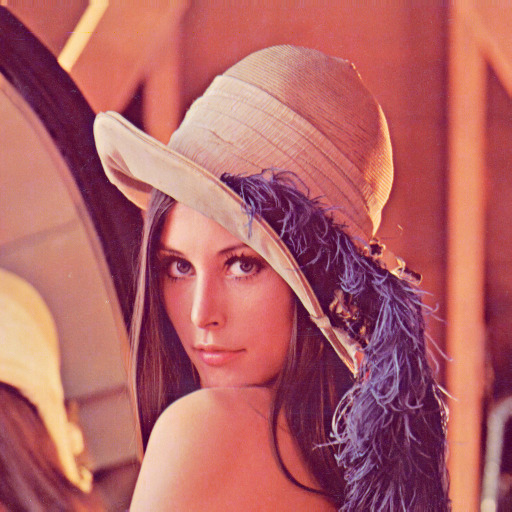
\includegraphics[height=8cm]{images/flip_horizontal.jpg}
            \caption{Obrázek po horizontálním zrcadlení}
        \end{subfigure}%
        ~
        \begin{subfigure}[t]{0.5\textwidth}
            \centering
            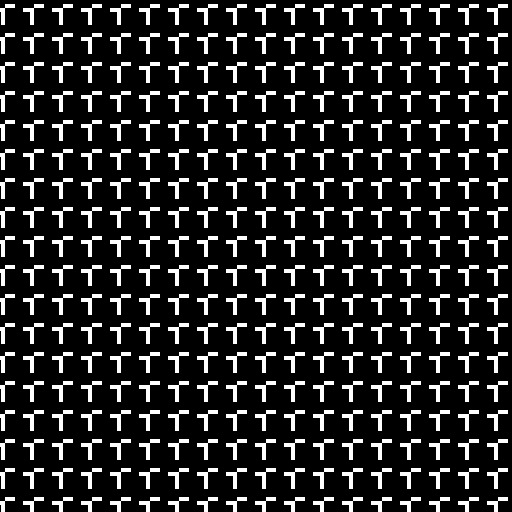
\includegraphics[height=8cm]{images/flip_horizontal_extracted.jpg}
            \caption{Extrahovaný obrázek}
        \end{subfigure}
        \caption{Vliv horizontálního zrcadlení na vodoznak v maximální hloubce}
    \end{center}
\end{figure*}

\begin{figure*}[h!]
    \begin{center}
        \begin{subfigure}[t]{0.5\textwidth}
            \centering
            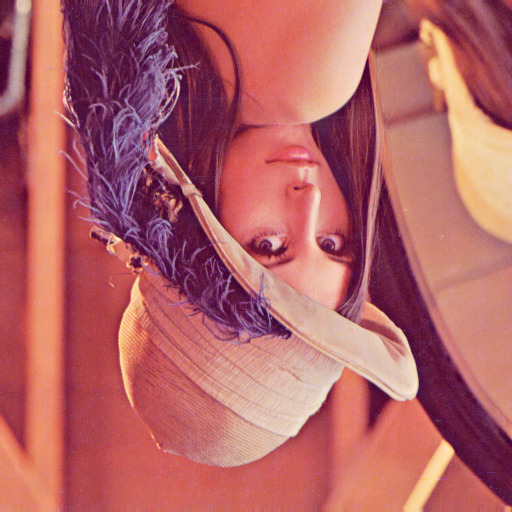
\includegraphics[height=8cm]{images/flip_vertical.jpg}
            \caption{Obrázek po vertikálním zrcadlení}
        \end{subfigure}%
        ~
        \begin{subfigure}[t]{0.5\textwidth}
            \centering
            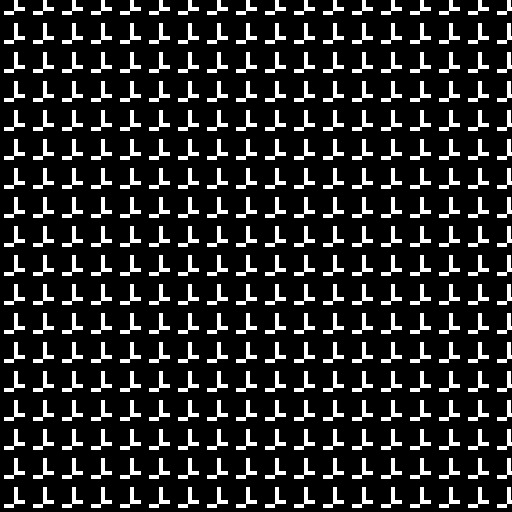
\includegraphics[height=8cm]{images/flip_vertical_extracted.jpg}
            \caption{Extrahovaný obrázek}
        \end{subfigure}
        \caption{Vliv vertikálního zrcadlení na vodoznak v minimální hloubce}
    \end{center}
\end{figure*}